%---------------------------------------------------------------------
%                          Cap\'itulo 4
%---------------------------------------------------------------------
\chapter{Aspectos operativos}
\section{Cronograma}
El cronograma planteado se puede ver en la figura \ref{fig:cronograma}

\begin{figure}[h]
    \centering
    \captionsetup{justification=centering}
    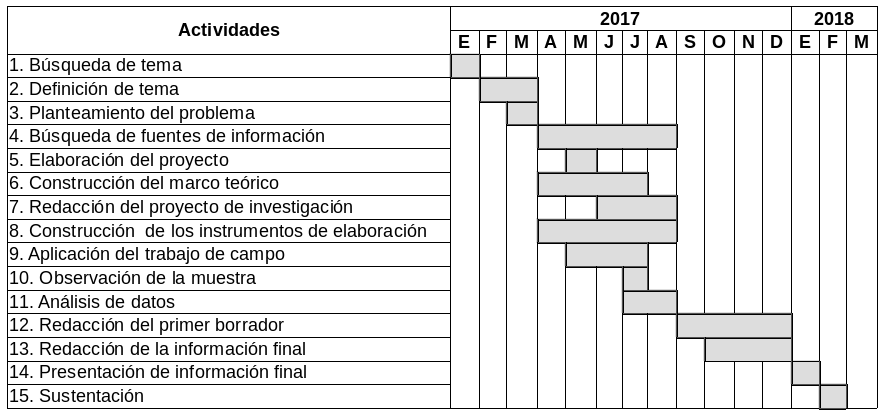
\includegraphics[width=1.0\textwidth]{Imagenes/Bitmap/cronograma}
    \caption{Cronograma de trabajo}
    \label{fig:cronograma}
\end{figure}

\section{Presupuesto y financiamiento}
El presupuesto para la realizaci\'on se puede ver en la tabla \ref{t:presupuesto}.
El financiamiento ser\'a asumido integramente por el tesista.

\begin{table}[]
  \centering
  \caption{Presupuesto}
  \label{t:presupuesto}
  \begin{tabular}{|p{5cm}|p{3cm}|p{3cm}|}
    \hline
    \thead{Detalle} & \thead{Prec. Unit.} & \thead{Sub Total} \\ \hline
    Material de escritorio &  &  \multicolumn{1}{|r|}{400.00} \\ \hline
    Anillados & \multicolumn{1}{|r|}{5.00}  &  \multicolumn{1}{|r|}{45.00} \\ \hline
    Copias &  &  \multicolumn{1}{|r|}{90.00} \\ \hline
    Adquisici\'on de bibliografia  &  & \multicolumn{1}{|r|}{400.00} \\ \hline
    Empastados &  \multicolumn{1}{|r|}{30.00}  & \multicolumn{1}{|r|}{90.00} \\ \hline
    Transporte &    & \multicolumn{1}{|r|}{100.00} \\ \hline
    Corrector de estilo &    & \multicolumn{1}{|r|}{300.00} \\ \hline
    Asesor estad\'istico &    & \multicolumn{1}{|r|}{300.00} \\ \hline
    Servicios (Internet) & \multicolumn{1}{|r|}{80.00} & \multicolumn{1}{|r|}{240.00} \\ \hline
    Elaboraci\'on de software   &  & \multicolumn{1}{|r|}{23 100.00} \\ \hline
    Aplicaci\'on de instrumentos  & \multicolumn{1}{|r|}{300.00} & \multicolumn{1}{|r|}{300.00} \\ \hline
    \textbf{TOTAL}  &  & \multicolumn{1}{|r|}{25 665.00} \\ \hline
  \end{tabular}
\end{table}

\section{Matriz de consistencia}
La matriz de consistencia de este trabajo se muestran en las tablas \ref{t:consistencia}
y \ref{t:consistencia_cont}.

\begin{sidewaystable}[htbp]
\centering
\caption{Matriz de consistencia}
\label{t:consistencia}
\begin{tabular}{|p{5cm}|p{5cm}|p{5cm}|p{4cm}|}
\hline
Problema & Objetivo & Hipotesis & Variables \\ \hline
\textbf{Problema general}

Cual es el efecto del uso de las herramientas de la computaci\'on en la nube
en la gesti\'on de las MiPYME pertenecientes al Centro de Desarrollo Empresarial
del Cusco.

\textbf{Problemas espec\'ificos}

\begin{enumerate}[noitemsep]
\item Cu\'al es el nivel de gesti\'on de las MiPYMES pertenecientes al Centro
de Desarrollo Empresarial del Cusco antes del uso de herramientas de la computaci\'on
en la nube.
\item Cu\'al es el nivel de gesti\'on de las MiPYMES pertenecientes al Centro
de Desarrollo Empresarial del Cusco despu\'es del uso de herramientas de la computaci\'on
en la nube.
\end{enumerate}
&
\textbf{Objetivo general}

Determinar el efecto del uso de la computaci\'on en la nube en la gesti\'on de
las micro, peque\~nas y medianas empresas pertenecientes al Centro de desarrollo
empresarial del Cusco.

\textbf{Objetivos espec\'ificos}
\begin{enumerate}
  \item Determinar el nivel de gesti\'on de las MiPYMES pertenecientes al Centro de
  Desarrollo Empresarial del Cusco antes del uso de las herramientas de la
  computaci\'on en la nube.
  \item Determinar el nivel de gesti\'on de las MiPYMES pertenecientes al Centro de
  Desarrollo Empresarial del Cusco despu\'es del uso de las herramientas de la
  computaci\'on en la nube.
\end{enumerate}
&
\textbf{Hip\'otesis general}

Existe un efecto positivo del uso de la computaci\'on en la nube en la
gesti'on de las micro, peque\~nas y medianas empresas pertenecientes al Centro de
Desarrollo Empresarial del Cusco.

\textbf{Hip\'otesis espec\'ificas}
\begin{enumerate}[noitemsep]
    % preguntaar si es necesario colocar las palabras pe-post implementacion
    \item El nivel de gesti\'on de las MiPYMES pertenecientes al Centro de Desarrollo
          Empresarial del Cusco antes del uso de las herramientas de la computaci\'on
          en la nube es deficiente.
    \item El nivel de gesti\'on de las MiPYMES pertenecientes al Centro de Desarrollo
          Empresarial del Cusco despu\'es del uso de las herramientas de la computaci\'on
          en la nube es eficiente.
    \item El efecto del uso de herramientas de la computaci'on en la nube en la
          gesti\'on de las MiPYMES pertenecientes al Centro de Desarrollo Empresarial
          del Cusco es positiva.
\end{enumerate}
&
La \'unica variable identificada es \textbf{Gesti\'on empresarial}.
\\ \hline
\end{tabular}
\end{sidewaystable}

% Please add the following required packages to your document preamble:
% \usepackage{graphicx}
\begin{sidewaystable}[]
\centering
\caption{Matriz de consistencia}
\label{t:consistencia_cont}
\resizebox{\textwidth}{!}{%
\begin{tabular}{|p{6cm}|p{4cm}|p{4cm}|}
\hline
Justificaci\'on & M\'etodo & Universo, poblaci\'on y muestra. \\ \hline
\textbf{Conveniencia}

Conocer el efecto del uso de las herramientas de la computaci\'on en la nube en
la gesti\'on de las MiPYME pertenecientes al Centro de Desarrollo Empresarial del Cusco y de esta forma
generar herramientas de apoyo a la gesti\'on lo que permitira lograr su crecimiento.

%% Incluir parrafos de

\textbf{Relevancia social}

Al realizar este estudio se implementaran e implantaran
herramientas de computaci\'on en la nube que permitiran mejorar los procesos de gesti\'on
m\'as importantes a un costo razonable que les permita desarrollarse y crecer.

\textbf{Implicancias pr'acticas}

Las herramientas que se implementaran en el presente trabajo mejorar\'an los procesos
de gesti\'on de las MiPYMEs pertenecientes al Centro de Desarrollo Empresarial del Cusco.

&
\textbf{Enfoque de investigaci\'on}

El enfoque para este trabajo ser\'a \emph{\textbf{cuantitatio}}.

\textbf{Alcance de investigaci\'on}

El estudio que se realizar\'a en el Centro de Desarrollo Empresarial del Cusco ser\'a
de \emph{\textbf{alcance explicativo}.}

\textbf{Disen\~no de investigaci\'on}

Debido a que el enfoque para este trabajo es cuantitativo, se deber\'a realizar
una \emph{\textbf{investigaci\'on experimental}} siendo el tipo espec\'ifico la
\emph{\textbf{preexperimental}}.
&
\textbf{Poblaci\'on y Muestra}

Empresas que son beneficiarias del Centro de Desarrollo Empresarial del Cusco.

\textbf{Tecnicas e instrumentos}

Las t\'ecnicas que se aplicar\'an para este trabajo ser\'an:
la \emph{\textbf{investigaci\'on documental}} e \emph{\textbf{investigaci\'on de campo}}
utilizando como instrumentos especificos las \emph{\textbf{fichas de trabajo}} y
\emph{\textbf{encuestas}}.

\textbf{M\'etodo estadisticos}

Para el an\'alisis de datos se utilizar\'a la \emph{\textbf{Prueba T de Student, Prueba
T-Student o Test-T}}, ya que es la que m\'as se adecua a nuestro escenario.

\\ \hline
\end{tabular}%
}
\end{sidewaystable}
%\section{Matriz de instrumentos}
%\section{Referencias bibliograficas}
%\section{Instrumentos de recolecci\'on de datos}
